
\subsection{Geometric Realization}

We wish to use expression graphs to generate linear maps by viewing the edges as
paths in a manifold equipped with an algebra-fibred bundle with connection,
taking their associated parallel transport maps, and combining these maps in a
pattern encoded in the expression graph. To accomplish this, we use the
following simple notion of geometric realization of graphs.

\begin{defn}[Geometric Graph]
A graph in a manifold $M$ or a geometric graph is a graph $G = (V, E)$ equipped
with a function $\gamma : E \to C^0(I, M)$, called a geometric realization of
$G$. We call $M$ the realizing manifold of $G$ under $\gamma$. For an edge from
$u$ to $v$ we write $\gamma_{u, v}$ to denote the path associated to that edge.
\end{defn}

\begin{rmk}
A geometric graph is essentially a collection of paths in a manifold but we
consider one or more copies of each path and ``identify'' their end-points in a
pattern encoded by a graph, even though these paths need not share end-points --
that is, we do not strictly require $\gamma_{u, v}(1) = \gamma_{v, w}(0)$. We
will see that this relaxation is essential to defining our notion of TQFTs. We
will ultimately be interested in expression graphs in manifolds, which will
provide us with a way to associate linear maps to manifolds.
\end{rmk}

\begin{exm}\label{exm:geomegraph}
Consider the graph in example \ref{exm:egraph1}. Then, we consider a mapping of
the edges to paths on a surface as shown below.\footnote{This diagram was
generated using \cite{Mathcha}.} Note that here we have
$\gamma_{u, v}(1) = \gamma_{v, w}(0)$ for most points but not all -- for
instance, $\gamma_{2, 3}$ and $\gamma_{3, 5}$ do not share any end-points.
\begin{figure}[H]
\begin{center}

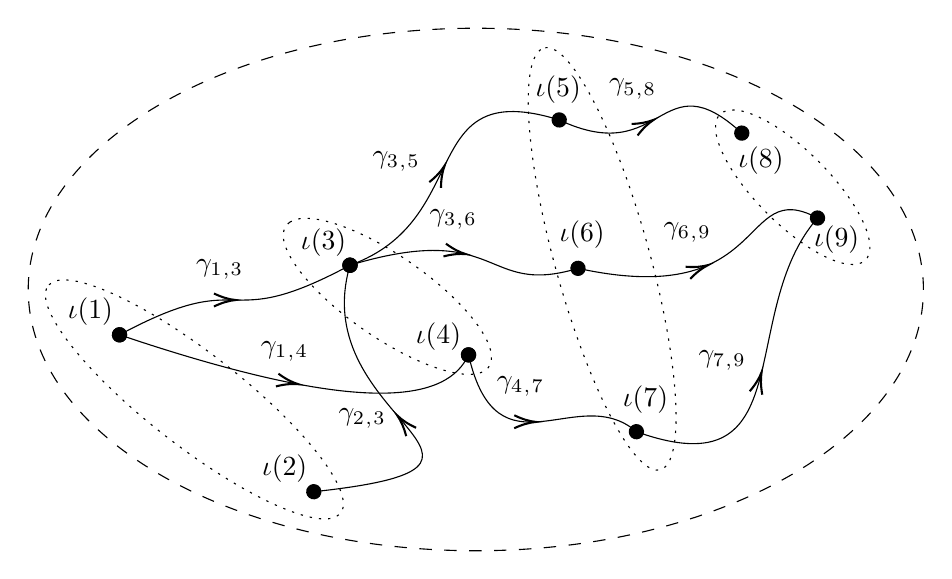
\begin{tikzpicture}[x=0.75pt,y=0.75pt,yscale=-0.95,xscale=0.95]
%uncomment if require: \path (0,281); %set diagram left start at 0, and has height of 281

%Shape: Ellipse [id:dp45216116111361904] 
\draw  [dash pattern={on 4.5pt off 4.5pt}] (6,138.5) .. controls (6,65.32) and (107.63,6) .. (233,6) .. controls (358.37,6) and (460,65.32) .. (460,138.5) .. controls (460,211.68) and (358.37,271) .. (233,271) .. controls (107.63,271) and (6,211.68) .. (6,138.5) -- cycle ;
%Curve Lines [id:da12378300176275903] 
\draw    (52.31,161.49) .. controls (119.1,125.59) and (102.4,162.09) .. (169.19,126.19) ;
\draw [shift={(169.19,126.19)}, rotate = 331.74] [color={rgb, 255:red, 0; green, 0; blue, 0 }  ][fill={rgb, 255:red, 0; green, 0; blue, 0 }  ][line width=0.75]      (0, 0) circle [x radius= 3.35, y radius= 3.35]   ;
\draw [shift={(111.13,143.84)}, rotate = 180.1] [color={rgb, 255:red, 0; green, 0; blue, 0 }  ][line width=0.75]    (10.93,-3.29) .. controls (6.95,-1.4) and (3.31,-0.3) .. (0,0) .. controls (3.31,0.3) and (6.95,1.4) .. (10.93,3.29)   ;
\draw [shift={(52.31,161.49)}, rotate = 331.74] [color={rgb, 255:red, 0; green, 0; blue, 0 }  ][fill={rgb, 255:red, 0; green, 0; blue, 0 }  ][line width=0.75]      (0, 0) circle [x radius= 3.35, y radius= 3.35]   ;
%Curve Lines [id:da3902364739215902] 
\draw    (169.19,126.19) .. controls (233.04,103.33) and (202.45,29.92) .. (275.29,52.51) ;
\draw [shift={(275.29,52.51)}, rotate = 17.23] [color={rgb, 255:red, 0; green, 0; blue, 0 }  ][fill={rgb, 255:red, 0; green, 0; blue, 0 }  ][line width=0.75]      (0, 0) circle [x radius= 3.35, y radius= 3.35]   ;
\draw [shift={(217.18,75.67)}, rotate = 476.11] [color={rgb, 255:red, 0; green, 0; blue, 0 }  ][line width=0.75]    (10.93,-3.29) .. controls (6.95,-1.4) and (3.31,-0.3) .. (0,0) .. controls (3.31,0.3) and (6.95,1.4) .. (10.93,3.29)   ;
\draw [shift={(169.19,126.19)}, rotate = 340.3] [color={rgb, 255:red, 0; green, 0; blue, 0 }  ][fill={rgb, 255:red, 0; green, 0; blue, 0 }  ][line width=0.75]      (0, 0) circle [x radius= 3.35, y radius= 3.35]   ;
%Curve Lines [id:da5125133831866234] 
\draw    (52.31,161.49) .. controls (178.45,204.05) and (218.84,194.46) .. (229.3,171.66) ;
\draw [shift={(229.3,171.66)}, rotate = 294.65] [color={rgb, 255:red, 0; green, 0; blue, 0 }  ][fill={rgb, 255:red, 0; green, 0; blue, 0 }  ][line width=0.75]      (0, 0) circle [x radius= 3.35, y radius= 3.35]   ;
\draw [shift={(142.99,186.54)}, rotate = 191.16] [color={rgb, 255:red, 0; green, 0; blue, 0 }  ][line width=0.75]    (10.93,-3.29) .. controls (6.95,-1.4) and (3.31,-0.3) .. (0,0) .. controls (3.31,0.3) and (6.95,1.4) .. (10.93,3.29)   ;
\draw [shift={(52.31,161.49)}, rotate = 18.65] [color={rgb, 255:red, 0; green, 0; blue, 0 }  ][fill={rgb, 255:red, 0; green, 0; blue, 0 }  ][line width=0.75]      (0, 0) circle [x radius= 3.35, y radius= 3.35]   ;
%Curve Lines [id:da9936282267570157] 
\draw    (150.83,241.06) .. controls (275.76,227.54) and (145.96,205.62) .. (169.19,126.19) ;
\draw [shift={(169.19,126.19)}, rotate = 286.3] [color={rgb, 255:red, 0; green, 0; blue, 0 }  ][fill={rgb, 255:red, 0; green, 0; blue, 0 }  ][line width=0.75]      (0, 0) circle [x radius= 3.35, y radius= 3.35]   ;
\draw [shift={(193.16,202.39)}, rotate = 409.89] [color={rgb, 255:red, 0; green, 0; blue, 0 }  ][line width=0.75]    (10.93,-3.29) .. controls (6.95,-1.4) and (3.31,-0.3) .. (0,0) .. controls (3.31,0.3) and (6.95,1.4) .. (10.93,3.29)   ;
\draw [shift={(150.83,241.06)}, rotate = 353.83] [color={rgb, 255:red, 0; green, 0; blue, 0 }  ][fill={rgb, 255:red, 0; green, 0; blue, 0 }  ][line width=0.75]      (0, 0) circle [x radius= 3.35, y radius= 3.35]   ;
%Curve Lines [id:da37329721640419344] 
\draw    (229.3,171.66) .. controls (243.97,235.64) and (284.76,184.82) .. (314.44,210.62) ;
\draw [shift={(314.44,210.62)}, rotate = 41] [color={rgb, 255:red, 0; green, 0; blue, 0 }  ][fill={rgb, 255:red, 0; green, 0; blue, 0 }  ][line width=0.75]      (0, 0) circle [x radius= 3.35, y radius= 3.35]   ;
\draw [shift={(263.43,205.67)}, rotate = 180.44] [color={rgb, 255:red, 0; green, 0; blue, 0 }  ][line width=0.75]    (10.93,-3.29) .. controls (6.95,-1.4) and (3.31,-0.3) .. (0,0) .. controls (3.31,0.3) and (6.95,1.4) .. (10.93,3.29)   ;
\draw [shift={(229.3,171.66)}, rotate = 77.09] [color={rgb, 255:red, 0; green, 0; blue, 0 }  ][fill={rgb, 255:red, 0; green, 0; blue, 0 }  ][line width=0.75]      (0, 0) circle [x radius= 3.35, y radius= 3.35]   ;
%Curve Lines [id:da6402293447536181] 
\draw    (169.19,126.19) .. controls (246.58,102.99) and (236.29,142.42) .. (284.82,127.77) ;
\draw [shift={(284.82,127.77)}, rotate = 343.19] [color={rgb, 255:red, 0; green, 0; blue, 0 }  ][fill={rgb, 255:red, 0; green, 0; blue, 0 }  ][line width=0.75]      (0, 0) circle [x radius= 3.35, y radius= 3.35]   ;
\draw [shift={(227.95,120.58)}, rotate = 190.98] [color={rgb, 255:red, 0; green, 0; blue, 0 }  ][line width=0.75]    (10.93,-3.29) .. controls (6.95,-1.4) and (3.31,-0.3) .. (0,0) .. controls (3.31,0.3) and (6.95,1.4) .. (10.93,3.29)   ;
%Curve Lines [id:da7275544623824886] 
\draw    (314.44,210.62) .. controls (399.23,240.98) and (364.55,150.12) .. (406.29,102.26) ;
\draw [shift={(406.29,102.26)}, rotate = 311.09] [color={rgb, 255:red, 0; green, 0; blue, 0 }  ][fill={rgb, 255:red, 0; green, 0; blue, 0 }  ][line width=0.75]      (0, 0) circle [x radius= 3.35, y radius= 3.35]   ;
\draw [shift={(377.94,180.41)}, rotate = 465.08] [color={rgb, 255:red, 0; green, 0; blue, 0 }  ][line width=0.75]    (10.93,-3.29) .. controls (6.95,-1.4) and (3.31,-0.3) .. (0,0) .. controls (3.31,0.3) and (6.95,1.4) .. (10.93,3.29)   ;
%Shape: Ellipse [id:dp21247917365246105] 
\draw  [color={rgb, 255:red, 0; green, 0; blue, 0 }  ,draw opacity=1 ][dash pattern={on 0.84pt off 2.51pt}] (16.54,136.11) .. controls (25.63,126.66) and (66.01,145.03) .. (106.72,177.14) .. controls (147.44,209.25) and (173.08,242.94) .. (163.99,252.39) .. controls (154.9,261.85) and (114.52,243.48) .. (73.81,211.37) .. controls (33.09,179.26) and (7.45,145.57) .. (16.54,136.11) -- cycle ;
%Curve Lines [id:da7880732583039812] 
\draw    (275.29,52.51) .. controls (328.72,77.63) and (326.15,20.9) .. (367.89,59.19) ;
\draw [shift={(367.89,59.19)}, rotate = 42.53] [color={rgb, 255:red, 0; green, 0; blue, 0 }  ][fill={rgb, 255:red, 0; green, 0; blue, 0 }  ][line width=0.75]      (0, 0) circle [x radius= 3.35, y radius= 3.35]   ;
\draw [shift={(323.24,52.43)}, rotate = 512.6] [color={rgb, 255:red, 0; green, 0; blue, 0 }  ][line width=0.75]    (10.93,-3.29) .. controls (6.95,-1.4) and (3.31,-0.3) .. (0,0) .. controls (3.31,0.3) and (6.95,1.4) .. (10.93,3.29)   ;
%Curve Lines [id:da726151739669847] 
\draw    (284.82,127.77) .. controls (383.33,149.3) and (366.22,80.72) .. (406.29,102.26) ;
\draw [shift={(350.78,126.12)}, rotate = 518.99] [color={rgb, 255:red, 0; green, 0; blue, 0 }  ][line width=0.75]    (10.93,-3.29) .. controls (6.95,-1.4) and (3.31,-0.3) .. (0,0) .. controls (3.31,0.3) and (6.95,1.4) .. (10.93,3.29)   ;
%Shape: Ellipse [id:dp20693904539608654] 
\draw  [color={rgb, 255:red, 0; green, 0; blue, 0 }  ,draw opacity=1 ][dash pattern={on 0.84pt off 2.51pt}] (138.62,104.37) .. controls (148.74,97.58) and (179.13,108.92) .. (206.48,129.69) .. controls (233.84,150.47) and (247.81,172.81) .. (237.69,179.59) .. controls (227.57,186.38) and (197.19,175.04) .. (169.83,154.27) .. controls (142.47,133.49) and (128.5,111.15) .. (138.62,104.37) -- cycle ;
%Shape: Ellipse [id:dp4442811176180146] 
\draw  [dash pattern={on 0.84pt off 2.51pt}] (268.26,15.88) .. controls (281.5,13.99) and (305.14,60.41) .. (321.05,119.55) .. controls (336.96,178.69) and (339.13,228.17) .. (325.89,230.05) .. controls (312.64,231.94) and (289.01,185.52) .. (273.09,126.38) .. controls (257.18,67.24) and (255.02,17.76) .. (268.26,15.88) -- cycle ;
%Shape: Ellipse [id:dp2537302094398456] 
\draw  [dash pattern={on 0.84pt off 2.51pt}] (358.5,48.46) .. controls (367.96,43.55) and (391.4,56.66) .. (410.84,77.74) .. controls (430.28,98.83) and (438.37,119.9) .. (428.91,124.82) .. controls (419.45,129.73) and (396.01,116.62) .. (376.57,95.54) .. controls (357.13,74.45) and (349.04,53.37) .. (358.5,48.46) -- cycle ;

% Text Node
\draw (50.31,158.09) node [anchor=south east] [inner sep=0.75pt]    {$\iota ( 1)$};
% Text Node
\draw (148.83,237.66) node [anchor=south east] [inner sep=0.75pt]    {$\iota ( 2)$};
% Text Node
\draw (168.57,122.92) node [anchor=south east] [inner sep=0.75pt]    {$\iota ( 3)$};
% Text Node
\draw (226.84,170.66) node [anchor=south east] [inner sep=0.75pt]    {$\iota ( 4)$};
% Text Node
\draw (262.03,45.25) node [anchor=south west] [inner sep=0.75pt]    {$\iota ( 5)$};
% Text Node
\draw (274.13,119.08) node [anchor=south west] [inner sep=0.75pt]    {$\iota ( 6)$};
% Text Node
\draw (306.28,202.6) node [anchor=south west] [inner sep=0.75pt]    {$\iota ( 7)$};
% Text Node
\draw (364.82,65) node [anchor=north west][inner sep=0.75pt]    {$\iota ( 8)$};
% Text Node
\draw (403.23,105) node [anchor=north west][inner sep=0.75pt]    {$\iota ( 9)$};
% Text Node
\draw (89.78,121.75) node [anchor=north west][inner sep=0.75pt]    {$\gamma _{1}{}_{,}{}_{3}$};
% Text Node
\draw (122.67,163.43) node [anchor=north west][inner sep=0.75pt]    {$\gamma _{1}{}_{,}{}_{4}$};
% Text Node
\draw (162.08,197.67) node [anchor=north west][inner sep=0.75pt]    {$\gamma _{2}{}_{,}{}_{3}$};
% Text Node
\draw (179.33,67.29) node [anchor=north west][inner sep=0.75pt]    {$\gamma _{3}{}_{,}{}_{5}$};
% Text Node
\draw (208.3,96.52) node [anchor=north west][inner sep=0.75pt]    {$\gamma _{3}{}_{,}{}_{6}$};
% Text Node
\draw (242.33,181.1) node [anchor=north west][inner sep=0.75pt]    {$\gamma _{4}{}_{,}{}_{7}$};
% Text Node
\draw (299.22,30.41) node [anchor=north west][inner sep=0.75pt]    {$\gamma _{5}{}_{,}{}_{8}$};
% Text Node
\draw (326.9,103.09) node [anchor=north west][inner sep=0.75pt]    {$\gamma _{6}{}_{,}{}_{9}$};
% Text Node
\draw (344.63,168.21) node [anchor=north west][inner sep=0.75pt]    {$\gamma _{7}{}_{,}{}_{9}$};


\end{tikzpicture}


\end{center}
\caption{A geometric graph}
\end{figure}
We notice that the same algebraic expression carries over:
\begin{align*}
        & (\gamma_{5, 8} \tensor (\gamma_{6, 9} \cwedge \gamma_{7, 9})) \\
  \circ & (\gamma_{3, 5} \tensor \gamma_{3, 6} \tensor \gamma_{4, 7}) \\
  \circ & ((\gamma_{3, 3} \cvee \gamma_{3, 3}) \tensor \gamma_{4, 4}) \\
  \circ & (\gamma_{3, 3} \tensor (\gamma_{4, 4} \boxtimes \gamma_{2, 3})) \\
  \circ & ((\gamma_{1, 3} \cvee \gamma_{1, 4}) \tensor \gamma_{2, 2})
\end{align*}
\end{exm}

At this point, we make a necessary observation. Consider geometric expression
graphs in a manifold equipped with an $A$--fibred bundle with connection. Then,
consider the expression of an expression graph realized in this manifold. If we
substitute the edges in the expression of the graph with the parallel transport
maps along the paths associated to the edges, we obtain a linear map from a
non-zero tensor power of $A$ to another such tensor power, given the graph has
at least one edge. However, there is no immediate way to obtain a map of the
form $\R \to A$ or $A \to \R$ in this method.

We recall that cobordisms $\varnothing \to S^1$ or
$S^1 \to \varnothing$ in $\Cob_2$ are given by composing cobordisms
$S^1 \to S^1$ with the following structures:
\[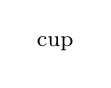
\begin{tikzpicture}[scale=0.5]
\cupcob{0, 2}
\node at (1.5, 0) (cuplbl) {{\footnotesize cup}};
\end{tikzpicture}
\qquad \qquad \qquad
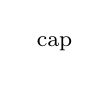
\begin{tikzpicture}[scale=0.5]
\capcob{3, 2}
\node at (1.5, 0) (caplbl) {{\footnotesize cap}};
\end{tikzpicture}\]
We would like analogous structures for expression graphs. We can use vertex
colouring to distinguish between copies of the empty manifold and copies of
$S^1$ in the result of the expression construction. So, we consider vertex
coloured expression graphs.
%Visually, loops
%attached to the source or target of an edge seem like possible candidates for
%these structures:
%\[\begin{tikzpicture}
%\node[circle, fill, inner sep=1.5pt] at (0, 0) (a) {};
%\node[circle, fill, inner sep=1.5pt] at (1, 0) (b) {};
%\draw[->] (a) [out=130, in=230, looseness=25] to (a);
%\midarrow{a}{b}
%\end{tikzpicture}
%\qquad \qquad \qquad
%\begin{tikzpicture}
%\node[circle, fill, inner sep=1.5pt] at (0, 0) (a) {};
%\node[circle, fill, inner sep=1.5pt] at (1, 0) (b) {};
%\draw[->] (b) [out=50, in=-50, looseness=25] to (b);
%\midarrow{a}{b}
%\end{tikzpicture}\]
%We will show that if we allow loops on vertices except for the ones which do not
%have any incoming or outgoing edges to begin with, then we can adapt the
%theory to this new setting.

%As a start, the expression construction algorithm is extended as follows:
%\begin{alg}
%Let $G$ be a graph where vertices, except for those without any edges from or to
%other vertices, can have loops. We then make the following modifications to $G$:
%\begin{enumerate}[(1)]
%\setlength{\itemsep}{0pt}
%
%\item Colour every vertex with a single colour -- say blue.
%
%\item If $u$ has no incoming edges except for a loop $(u, u)$ but has outgoing
%edges, then we add another copy $u'$ of $u$, color it green, add the edge
%$(u', u)$ and delete the loop $(u, u)$.
%\[\begin{tikzpicture}
%\node[circle, fill, inner sep=1.5pt, color=blue] at (0, 0) (a) {};
%\node[circle, fill, inner sep=1.5pt, color=blue] at (1, 0.5) (b1) {};
%\node[circle, fill, inner sep=1.5pt, color=blue] at (1, -0.5) (bn) {};
%\midarrow{a}{b1}
%\midarrow{a}{bn}
%\draw[->] (a) [out=130, in=230, looseness=15] to (a);
%\draw[loosely dotted, thick] (b1) -- (bn);
%\end{tikzpicture}
%\qquad
%\begin{tikzpicture}
%\node at (0, 0.5)   (TOP)     {};
%\node at (0, 0)   (TO)      {$\Longrightarrow$};
%\node at (0, -0.5)  (BOTTOM)  {};
%\end{tikzpicture}
%\qquad
%\begin{tikzpicture}
%\node[circle, fill, inner sep=1.5pt, color=green!55!black] at (0, 0) (a1) {};
%\node[circle, fill, inner sep=1.5pt, color=blue] at (1, 0) (a2) {};
%\node[circle, fill, inner sep=1.5pt, color=blue] at (2, 0.5) (b1) {};
%\node[circle, fill, inner sep=1.5pt, color=blue] at (2, -0.5) (bn) {};
%\midarrow{a1}{a2}
%\midarrow{a2}{b1}
%\midarrow{a2}{bn}
%\draw[loosely dotted, thick] (b1) -- (bn);
%\end{tikzpicture}\]
%
%\item If $u$ has incoming edges but no outgoing edges except for a loop
%$(u, u)$, then we add a green copy $u'$ of $u$ as before, add the edge $(u, u')$
%and delete the loop $(u, u)$.
%\[\begin{tikzpicture}
%\node[circle, fill, inner sep=1.5pt, color=blue] at (0, 0) (a) {};
%\node[circle, fill, inner sep=1.5pt, color=blue] at (-1, 0.5) (b1) {};
%\node[circle, fill, inner sep=1.5pt, color=blue] at (-1, -0.5) (bn) {};
%\midarrow{b1}{a}
%\midarrow{bn}{a}
%\draw[->] (a) [out=50, in=-50, looseness=15] to (a);
%\draw[loosely dotted, thick] (b1) -- (bn);
%\end{tikzpicture}
%\qquad
%\begin{tikzpicture}
%\node at (0, 0.5)   (TOP)     {};
%\node at (0, 0)   (TO)      {$\Longrightarrow$};
%\node at (0, -0.5)  (BOTTOM)  {};
%\end{tikzpicture}
%\qquad
%\begin{tikzpicture}
%\node[circle, fill, inner sep=1.5pt, color=green!55!black] at (0, 0) (a1) {};
%\node[circle, fill, inner sep=1.5pt, color=blue] at (-1, 0) (a2) {};
%\node[circle, fill, inner sep=1.5pt, color=blue] at (-2, 0.5) (b1) {};
%\node[circle, fill, inner sep=1.5pt, color=blue] at (-2, -0.5) (bn) {};
%\midarrow{a2}{a1}
%\midarrow{b1}{a2}
%\midarrow{bn}{a2}
%\draw[loosely dotted, thick] (b1) -- (bn);
%\end{tikzpicture}\]
%
%\item If $u$ has both incoming and outgoing edges along with a loop $(u, u)$,
%we replace the loop with a path $u, u', u''$, where $u'$ is a green copy of $u$
%and $u''$ is another blue copy of $u$.
%\[\begin{tikzpicture}
%\node[circle, fill, inner sep=1.5pt, color=blue] at (0, 0) (a) {};
%\node[circle, fill, inner sep=1.5pt, color=blue] at (1, 0.35) (b1) {};
%\node[circle, fill, inner sep=1.5pt, color=blue] at (1, -0.35) (bn) {};
%\node[circle, fill, inner sep=1.5pt, color=blue] at (-1, 0.35) (c1) {};
%\node[circle, fill, inner sep=1.5pt, color=blue] at (-1, -0.35) (cn) {};
%\midarrow{a}{b1}
%\midarrow{a}{bn}
%\draw[->] (a) [out=60, in=120, looseness=15] to (a);
%\midarrow{c1}{a}
%\midarrow{cn}{a}
%\draw[loosely dotted, thick] (b1) -- (bn);
%\draw[loosely dotted, thick] (c1) -- (cn);
%\end{tikzpicture}
%\qquad
%\begin{tikzpicture}
%\node at (0, 0.35)   (TOP)     {};
%\node at (0, 0)   (TO)      {$\Longrightarrow$};
%\node at (0, -0.35)  (BOTTOM)  {};
%\end{tikzpicture}
%\qquad
%\begin{tikzpicture}
%\node[circle, fill, inner sep=1.5pt, color=blue] at (-1, 0) (a1) {};
%\node[circle, fill, inner sep=1.5pt, color=green!55!black] at (0, 0) (a2) {};
%\node[circle, fill, inner sep=1.5pt, color=blue] at (1, 0) (a3) {};
%\node[circle, fill, inner sep=1.5pt, color=blue] at (2, 0.35) (b1) {};
%\node[circle, fill, inner sep=1.5pt, color=blue] at (2, -0.35) (bn) {};
%\node[circle, fill, inner sep=1.5pt, color=blue] at (-2, 0.35) (c1) {};
%\node[circle, fill, inner sep=1.5pt, color=blue] at (-2, -0.35) (cn) {};
%\midarrow{a3}{b1}
%\midarrow{a3}{bn}
%\midarrow{c1}{a1}
%\midarrow{cn}{a1}
%\midarrow{a1}{a2}
%\midarrow{a2}{a3}
%\draw[loosely dotted, thick] (b1) -- (bn);
%\draw[loosely dotted, thick] (c1) -- (cn);
%\end{tikzpicture}\]
%
%\item If $G$ is a disjoint union $\coprod_i G_i$ and some $G_i = \varnothing$,
%we replace $G_i$ with an edge $(u_{G_i}, v_{G_i})$, where both the vertices are
%green:
%\[\begin{tikzpicture}
%\node at (0, 0) (a) {$\varnothing$};
%\end{tikzpicture}
%\qquad
%\begin{tikzpicture}
%\node at (0, 0)   (TO)      {$\Longrightarrow$};
%\end{tikzpicture}
%\qquad
%\begin{tikzpicture}
%\node[circle, fill, inner sep=1.5pt, color=green!55!black] at (0, 0) (a1) {};
%\node[circle, fill, inner sep=1.5pt, color=green!55!black] at (2, 0) (a3) {};
%\midarrow{a1}{a3}
%\end{tikzpicture}\]
%\begin{rmk}
%This is a case we ignored in the first expression construction aglorithm -- we
%did so for simplicity. We handle this now because we now have a way to deal with
%empty sources and targets.
%\end{rmk}
%
%\item We apply the steps of the first expression construction algorithm with
%copied vertices having the same colour as the original.
%
%\item We then identify green vertices with the empty manifold and obtain our
%expression from the identification of the graph in its final state with some
%cobordism in $\Cob_2$.
%
%\end{enumerate}
%\end{alg}

%Disjoint unions are easily adapted as well. However, we will change our
%definitions of source and target expression graphs since we will now interpret
%looped vertices as cobordisms of the empty manifold. We first adapt expression
%graphs to include loops.

\begin{defn}[Pretransport Graph]
A pretransport graph is an expression graph $G$ with a colour function
$V(G) \to \set{{\color{green!55!black}\text{green}},
{\color{blue!55!black}\text{blue}}}$ (with no constraints on adjacency of
vertices).
\end{defn}

\begin{defn}[Pretransport Homomorphism]
A pretransport homomorphism is a colour-preserving expression homomorphism.
\end{defn}

%\begin{rmk}
%We note that pretransport homomorphisms, being graph homomorphisms must preserve
%loops.
%\end{rmk}

From \ref{cor:expiso_unique}, it is immediate that:

\begin{cor}
Pretransport isomorphisms are unique.
\end{cor}

We now redefine the source and target of a pretransport graph so that
constructions like expressions and gluing can be adapted to this new setting
where we allow empty graphs to be sources and targets.

\begin{defn}
Let $G$ be a pretransport graph with $s_1, \dots, s_n$ the ordering of the
source vertices of its underlying expression graph and $t_1, \dots, t_m$ the
ordering of the target vertices thereof. Let $s_{i_1}, \dots, s_{i_p}$ be the
green source vertices and $t_{j_1}, \dots t_{j_q}$ be the green target vertices
in $G$. Then, the source of $G$ is defined to be the expression graph
\[
  S(G) := \set{s_1, \dots, s_{i_1 - 1}}
       \amalg \varnothing
       \amalg \set{s_{i_1 + 1}, \dots, s_{i_2}}
       \amalg \varnothing
       \amalg \cdots
       \amalg \varnothing
       \amalg \set{s_{i_p + 1}, \dots, s_{n}}
\]
The target of $G$ is defined to be the expression graph
\[
  T(G) := \set{t_{1}, \dots, t_{j_1 - 1}}
       \amalg \varnothing
       \amalg \set{t_{j_1 + 1}, \dots, t_{j_2}}
       \amalg \varnothing
       \amalg \cdots
       \amalg \varnothing
       \amalg \set{t_{j_q + 1}, \dots, t_{m}}
\]
\end{defn}

\begin{defn}
Gluing of expression graphs extends to gluing of pretransport graphs if we
consider pretransport isomorphisms instead of expression isomorphisms. More
precisely, for pretransport graphs $G$ and $H$, if $S(H) \cong T(G)$, then the
gluing is exactly the same as for expression graphs except for positions where
we have instances of $\varnothing$. For this, we have the following cases:
\begin{enmrt}
\li $H$ and $G$ both have green vertices at that position: we glue them
as usual.
\li $H$ has a green vertex but $G$ has $\varnothing$: we simply forget
that $G$ has $\varnothing$.
\li $H$ has $\varnothing$ but $G$ has a green vertex: we forget the copy
of $\varnothing$
\li $H$ and $G$ both have copies of $\varnothing$: we keep a single copy
of $\varnothing$
\end{enmrt}
\end{defn}

\begin{defn}[Expression Construction]
The expression of a pretransport graph $G$ is obtained by running the expression
construction on $G$ by forgetting colours and then identifying green vertices
with the empty manifold in the resulting cobordism in $\Cob_2$.
\end{defn}

We then consider the class of graphs that will yield our desired linear maps.

\begin{defn}[Transport Graph]
We call a geometric pretransport graph a transport graph.
\end{defn}

\begin{defn}[Geometric Homomorphism]
Let $G$ and $H$ be graphs in manifolds $M$ and $N$ with geometric realizations
$\gamma^G$ and $\gamma^H$ respectively, then a homomorphism $h : G \to H$
equipped with a smooth map $f : M \to N$ making the following diagram commute is
called a geometric homomorphism:
\[\begin{tikzpicture}[baseline=(a).base]
\node[scale=\diagscale] (a) at (0, 0){
\begin{tikzcd}
E(G) \ar[d, "\gamma^G" left] \ar[r, "h" above] &
E(H) \ar[d, "\gamma^H" right] \\
C^0(I, M) \ar[r, "f_*" below] &
C^0(I, N)
\end{tikzcd}
};
\end{tikzpicture}\]
where $f_*$ is the post-composition map $g \mapsto f \circ g$, and the
homomorphism $h$ is viewed as the function it induces on edge sets.
\end{defn}

\begin{defn}[Transport Homomorphism]
A geometric pretransport homomorphism is called a transport homomorphism.
\end{defn}

Pasting commutative squares as the one above along the $\gamma$ sides, we
observe that geometric homomorphisms compose associatively. Taking
$h$ and $f$ as the identity maps yields an identity morphism of geometric
graphs. Similarly, transport homomorphism also compose associatively and have
units. Furthermore, transport graphs inherit the disjoint union from their
underlying expression graphs and manifolds. For their gluing, we require a
notion of gluing geometric realizations.

We first observe that if $G$ and $H$ are transport graphs with a transport
isomorphism $S(H) \to T(G)$, it is unique by \ref{cor:expiso_unique}, since
there is only one map of path sets -- the empty map which always makes the
rquired diagram commute. We then have the following basic fact.

\begin{cor}
Let $G$ and $H$ be transport graphs realized in manifolds
$M$ and $N$ with geometric realizations $\gamma^G$ and
$\gamma^H$ respectively such that $\psi_{G, H} : S(H) \to T(G)$ is a unique
pretransport homomorphism, and $M$ and $N$ are ``smoothly gluable'' at some
part. Then, there exists a geometric realization
\[
  \gamma^H * \gamma^G : E(H * G) \to C^0(I, N * M)
\]
of the pretransport graph $H * G$ in $N * M$.
\end{cor}
\begin{proof}
We can define $\gamma^H * \gamma^G$ piecewise since the gluing site has no
edges.
\end{proof}

\begin{defn}[Gluing Transport Graphs]
For transport graphs $(G, \gamma^G)$ and $(H, \gamma^H)$ with $S(H) \cong T(G)$
with a transport homomorphism, we define their gluing in the obvious way:
\[
  (H, \gamma^H) * (G, \gamma^G) := (H * G, \gamma^H * \gamma^G)
\]
\end{defn}

This is enough structure to develop a simple system for doing algebra using
paths on a manifold. In particular, it yields at least two monoidal double
categories of transport graphs realized in manifolds. We develop one of these
notions of TQFTs next.
\TODO{I am not sure if it is appropriate call this a notion of TQFTs.}

